\section{Method Details}
\label{xsec:method_details}

\subsection{QA Construction}
\label{xsubsec:details_of_qa_construction}

\subsubsection{Prompt Template for QA Generation}

% \begin{figure}[htbp]
\begin{tcolorbox}[colback=gray!5]
\small
\textbf{[System]}\\ 
You are an expert in document question-answering dialogue synthesis. Please complete the following instructions based on the given text. The response must be true and accurate, and no additional content should be output. \\

\textbf{[Task Description]}\\
Your task is \textcolor{blue}{<detailed\_task\_description>}\\

\textbf{[Restriction]} \\
Ensure questions and answers are suitable and correct.

Only include questions that have definite answers, that is:
\begin{itemize}[leftmargin=*]
    \item one can see the content in the image that the question asks about and can answer confidently;
    \item one can determine confidently from the image that it is not in the image, don't ask any question that cannot be answered confidently.
\end{itemize}

Provide detailed evidence description first and then give final short answers. Use examples or reasoning steps to support your content. You can include multiple paragraphs if necessary.

\textcolor{blue}{<other\_restriction\_description>} \\


\textbf{[Response Examples]}\\
\textcolor{blue}{<few\_qa\_examples>} \\

\textbf{[Context Input]}\\
\textcolor{blue}{<structured\_text> | <previous\_response>} \\

\label{text:prompt_template_qa_construction}
\end{tcolorbox}
% \caption{Prompt template for quention}
% \label{fig:answer_extraction}
% \end{figure}

Notes: \textcolor{blue}{<structured\_text>} refers to \textbf{text-type-bbox} triple processed by Docmind engine, which is discussed in detail in \Cref{subsubsec:evidence_collection}. \textcolor{blue}{<previous\_response>} refers to possible intermediate result(\eg, summary sentences in our Para-Title \Locating~task. Specifically, we prompt LVLMs to generate summary sentences of one or multiple paragraphs under certain section titles first, and then utilize these summaries and title names to construct question-answering data.)



\subsubsection{Prompt Template for QA Verification}

\begin{tcolorbox}[colback=gray!5]
\small
\textbf{[System]}\\ 
You are an expert in document question-answering verification. Please complete the following instructions based on the given text. The response must be true and accurate, and no additional content should be output. \\

\textbf{[Task description \& Verification criteria]} \\ 
Your task is to ensure the quality of question-answer pairs in the context provided. you need to follow the steps outlined below to systematically evaluate each pair's effectiveness and accuracy. Implement this process diligently to maintain high standards across the batch of QA pairs. \\

1. Question type check \\

Does the question match the task description: \textcolor{blue}{<task\_description>}

Make sure the question meets the required task context. \\

2. Formatting and Presentation \\

Is answer properly formatted?

Ensure the answer uses a list format to store the title content. \\

3. Relevance Check \\
Does the question relate directly to document content rely on the context provided, the answer accurately reflect the information in the document?

Ensure the question is formulated based on information explicitly stated or implied in the document. The question should not introduce concepts unrelated to the document's content. 

Validate that the answer references specific data or statements from the document. Avoid including extraneous information not supported by the document. \\

4. Clarity and Precision \\
Is the question clear and unambiguous? And is the answer concise and precise?
Ensure the language is straightforward and easily understandable, avoid complex phrasing that may confuse the reader.

The intention of the question and answer pair must be clear and direct, avoiding verbosity and unnecessary detail.

Ensure the answer fully addresses the question without omitting crucial information. \\

5. Consistency and Coherence \\
Check for logical flow and coherence, ensuring the question aligns seamlessly with the document's narrative or arguments. Verify that the answer does not contradict or misrepresent other sections of the document.

By practicing this process, you can confirm whether the quality of the question-answer pairs meets the requirements. If all the above conditions are met, please output yes, otherwise output no. \\

Generated QA: \textcolor{blue}{<qa>} \\

Input Context: \textcolor{blue}{<evidence\_context>}

\label{text:prompt_template_qa_verification}
\end{tcolorbox}

\begin{figure*}
    \centering
    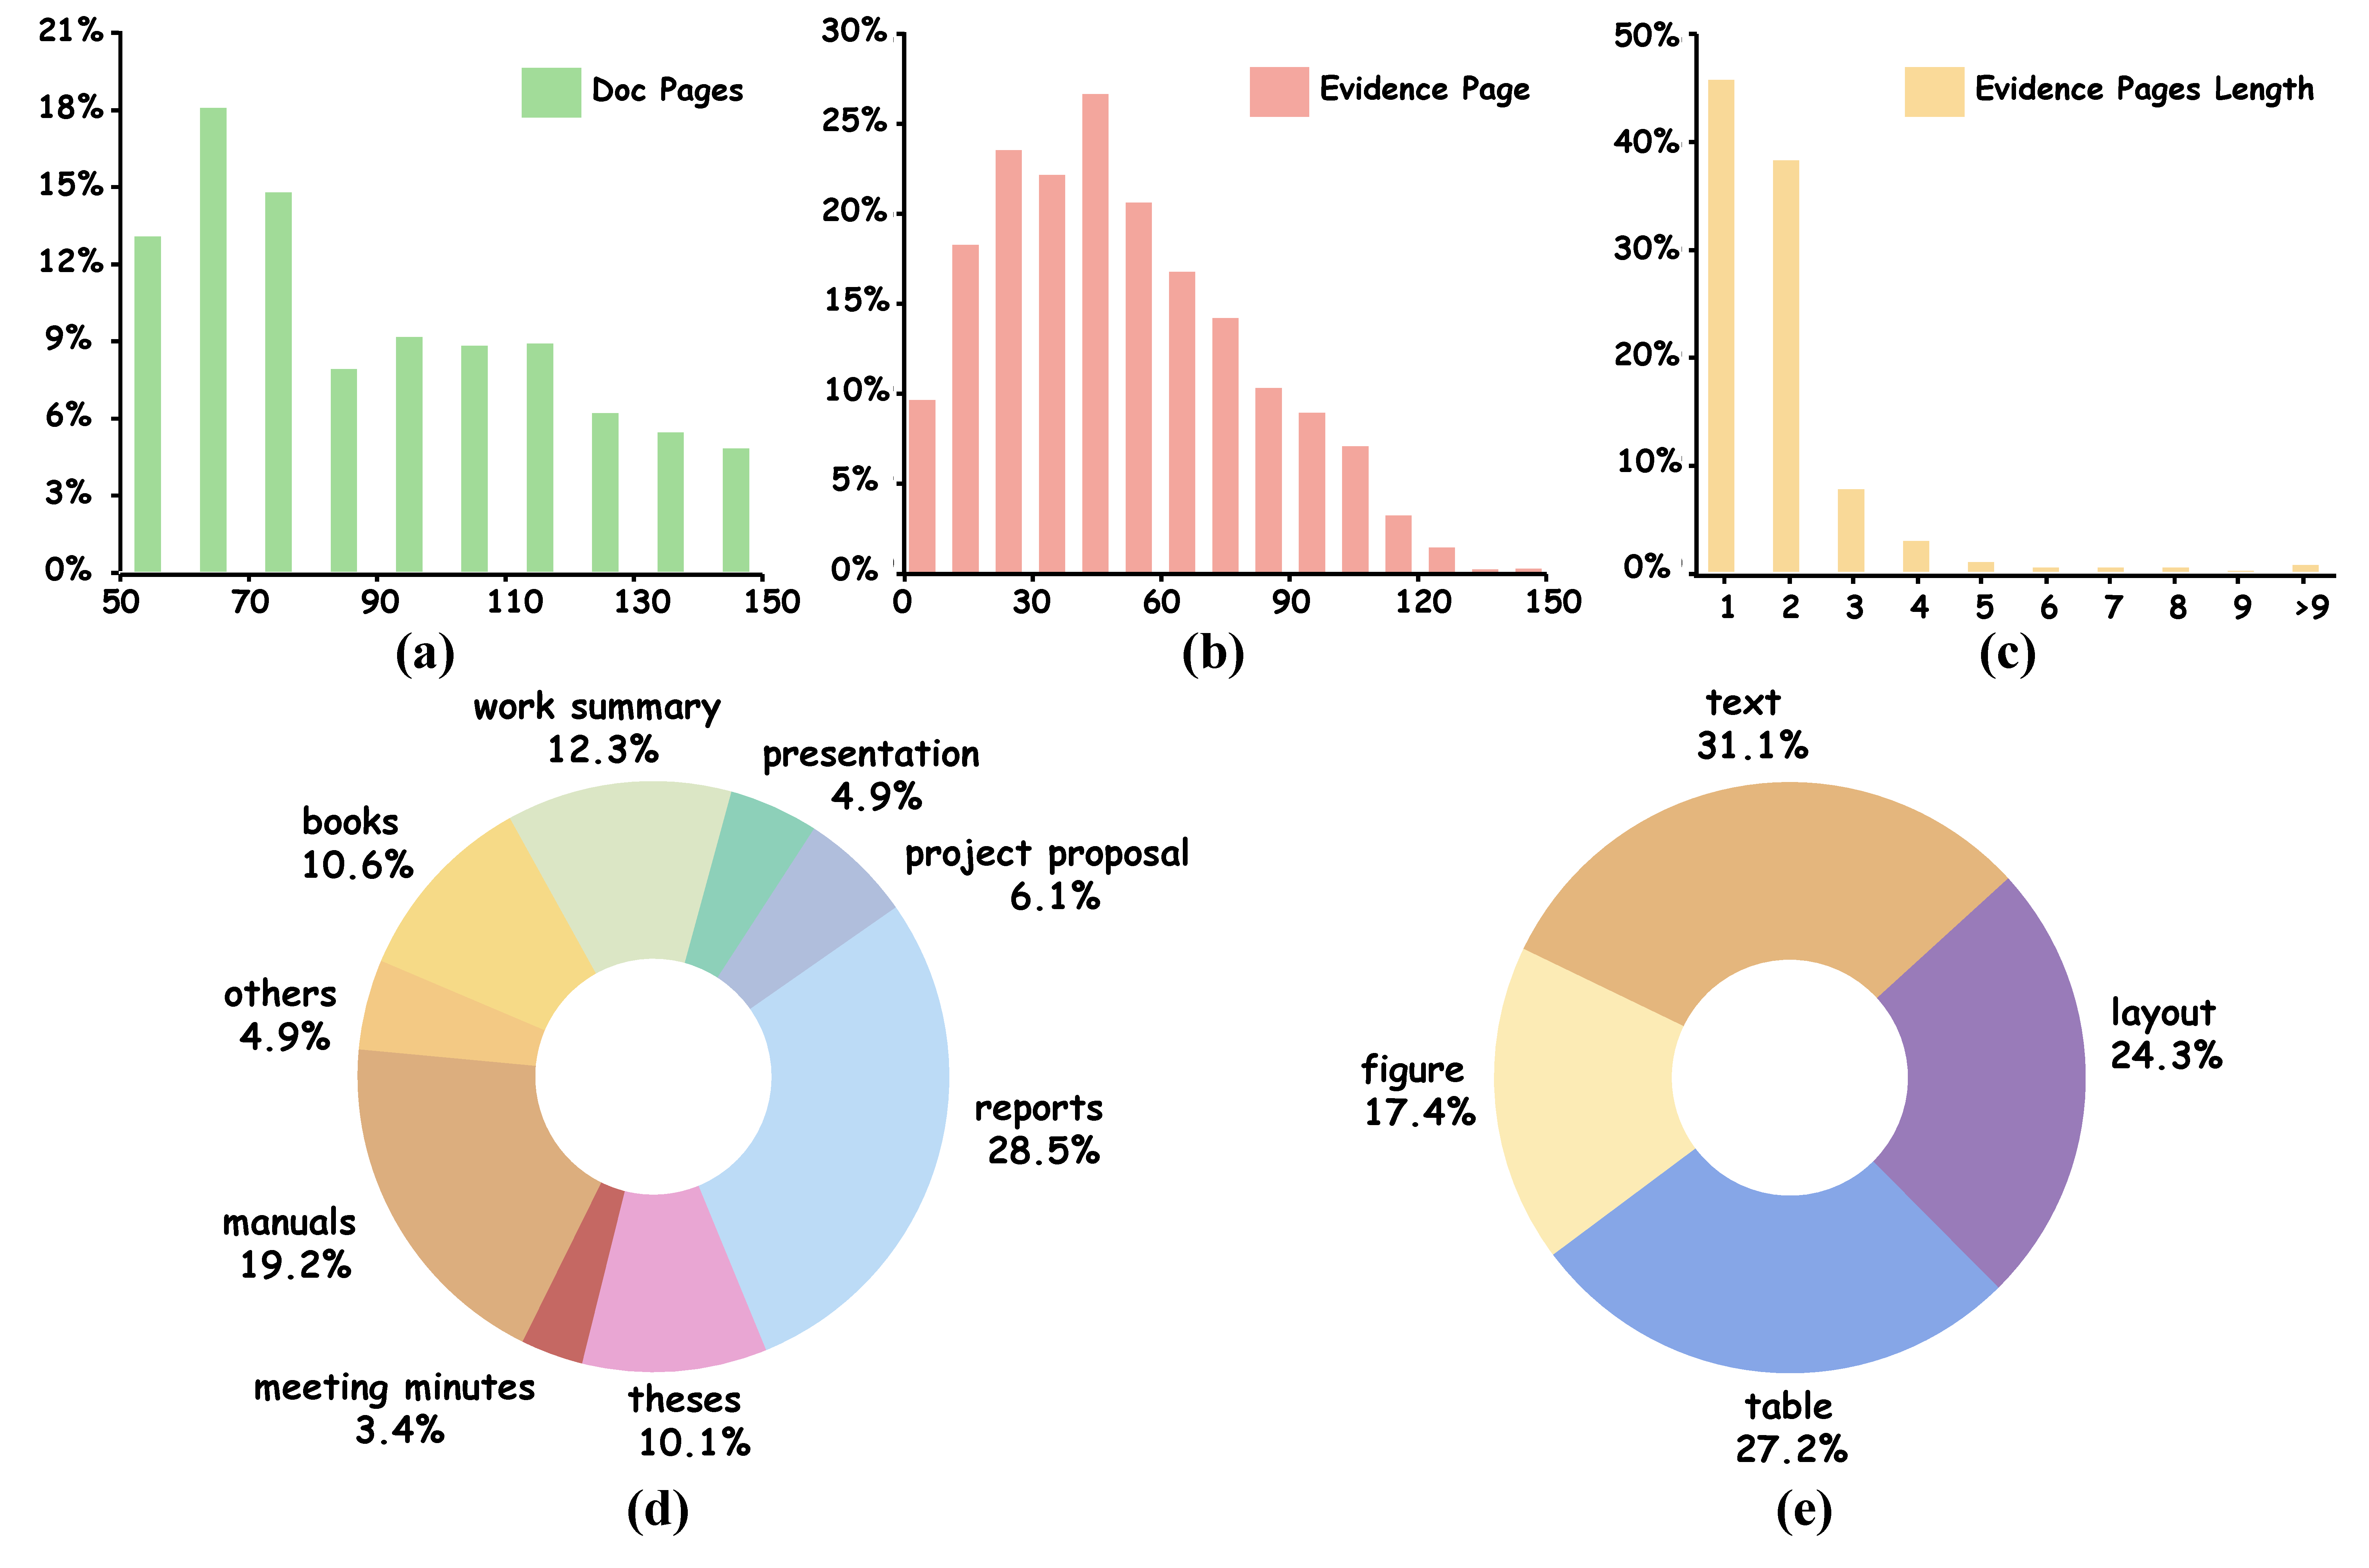
\includegraphics[width=0.9\textwidth]{img/statis_merge_1215.pdf} % 调整宽度
    \caption{The statistical analysis of our dataset about the distribution characteristics across (a) \textbf{document pages}, (b) \textbf{answer evidence page}, (c) \textbf{evidence pages length}, (d) \textbf{document sources}, and (e) \textbf{evidence element types}.}
    \label{fig:document_distribution}
\end{figure*}


\subsubsection{Statistics of QA Verification}
\label{xsubsubsec:statistics_of_qa_verification}
\begin{table}[htbp]
    \centering
    % \small
    % \footnotesize
    \scriptsize
    \vspace{-1.0mm}
    \resizebox{0.4\textwidth}{!}{
        \begin{tabular}{@{}l@{\hspace{15mm}}c@{\hspace{15mm}}c@{}}
        \toprule
        \textbf{Verify}  & \textbf{U + R}       & \textbf{L} \\
        
        \midrule
        \textbf{Before} & 2857 & 1520 \\
        \textbf{After} & 1630 & 695 \\                               
        &57.1\%↓   &45.7\%↓ \\            
        \bottomrule
        \end{tabular}}
    \caption{Statistics of changes in the amount of data before and after verification.}
    \label{tab:qa_numeric_verification}
    \vspace{-5mm}
\end{table}